%%%%%%%%%%%%%%%%%%%%%%%%%%%%%%%%%%%%%%%%%%%%%%%%%%%%%%%%%%%%%%%%%%%%
%% I, the copyright holder of this work, release this work into the
%% public domain. This applies worldwide. In some countries this may
%% not be legally possible; if so: I grant anyone the right to use
%% this work for any purpose, without any conditions, unless such
%% conditions are required by law.
%%%%%%%%%%%%%%%%%%%%%%%%%%%%%%%%%%%%%%%%%%%%%%%%%%%%%%%%%%%%%%%%%%%%

\documentclass{beamer}
\usetheme[logo=figures/CASCON_LOGO]{fibeamer}
\usepackage[utf8]{inputenc}
\usepackage[
  main=english, %% By using `czech` or `slovak` as the main locale
                %% instead of `english`, you can typeset the
                %% presentation in either Czech or Slovak,
                %% respectively.
  czech, slovak %% The additional keys allow foreign texts to be
]{babel}        %% typeset as follows:
%%
%%   \begin{otherlanguage}{czech}   ... \end{otherlanguage}
%%   \begin{otherlanguage}{slovak}  ... \end{otherlanguage}
%%
%% These macros specify information about the presentation
\title{\normalsize Stochastic Algorithms for Instruction Scheduling and Rapid Prototyping In Coconut} %% that will be typeset on the
\subtitle{Presented By: Curtis D'Alves} %% title page.
\author{Authors: Curtis D'Alves, Christopher Anand, Wolfram Kahl, William
  O'Farrell, Robert Enenkal, James You}
%% These additional packages are used within the document:
\usepackage{ragged2e}  % `\justifying` text
\usepackage{booktabs}  % Tables
\usepackage{tabularx}
% \usepackage{tikz}      % Diagrams
% \usetikzlibrary{calc, shapes, backgrounds}
\usepackage{amsmath, amssymb}
\usepackage{url}       % `\url`s
\usepackage{listings}  % Code listings
\usepackage{float}
\usepackage{caption}
\usepackage[cache=false]{minted}
% \lstset{
% 	tabsize=4,
% 	language=Haskell,
%         basicstyle=\scriptsize,
%         upquote=true,
%         aboveskip={1.5\baselineskip},
%         columns=fixed,
%         showstringspaces=false,
%         extendedchars=true,
%         breaklines=true,
%         prebreak = \raisebox{0ex}[0ex][0ex]{\ensuremath{\hookleftarrow}},
%         frame=single,
%         showtabs=false,
%         showspaces=false,
%         showstringspaces=false,
%         identifierstyle=\color[rgb]{0,0.7,0.7},
%         keywordstyle=\color[rgb]{0.7,0,0.7},
%         commentstyle=\color[rgb]{1,0,0},
%         stringstyle=\color[rgb]{0.4,0.4,0.4}
%       }

\lstset{
  frame=none,
  xleftmargin=2pt,
  stepnumber=1,
  numbers=left,
  numbersep=5pt,
  numberstyle=\ttfamily\tiny\color[gray]{0.3},
  belowcaptionskip=\bigskipamount,
  captionpos=b,
  escapeinside={*'}{'*},
  language=haskell,
  tabsize=2,
  emphstyle={\bf},
  commentstyle=\it,
  stringstyle=\mdseries\rmfamily,
  showspaces=false,
  keywordstyle=\bfseries\rmfamily,
  columns=flexible,
  basicstyle=\small\sffamily,
  showstringspaces=false,
  morecomment=[l]\%,
}

\frenchspacing
\begin{document}
  \frame{\maketitle}

  \AtBeginSection[]{% Print an outline at the beginning of sections
    \begin{frame}<beamer>
      \frametitle{Table of Contents}
      \tableofcontents[currentsection]
    \end{frame}}

  \begin{darkframes}

    \section{Introduction}

    \subsection{Instruction Scheduling}
    \begin{frame}{Instruction Scheduling}
      
      \alert{ \bf Problem:} Given a set of instructions and dependencies, designate an order (find a {\it schedule}) satisfying the dependencies and optimizing performance
      \qquad \\
      \qquad \\
      \qquad \\
      Known {\bf \color{green} NP-Complete} problem, practically solved by
      \begin{itemize}
      \item Heuristics
      \item Approximation Algorithms
      \end{itemize}
    \end{frame}
    
    \begin{frame}{Types of Scheduling}

      \begin{itemize}
      \item {\bf \color{green} Basic Block:} break code into blocks within branches {\bf \alert{(most commonly performed scheduling)}} \\
        \qquad \\

      \item {\bf \color{green} Global Scheduling:} schedule across basic block boundaries \\
        \qquad \\

      \item {\bf \color{green} Modulo Scheduling:} an algorithm to increase pipelining of loops by interleaving different iterations \\
        \qquad \\

      \item {\bf \color{green} Trace Scheduling:} tries to optimize control flow by predicting routes taken on branches
      \end{itemize}
    \end{frame}

    \begin{frame}{Register Allocation}

	{\bf \alert{ Problem:}} Given a schedule, assign registers keeping in mind
	\begin{itemize}
		\item limited \# of registers
		\item can't rewrite a register until consumed by dependent instructions
	\end{itemize}
	\qquad \\
	\qquad \\
	Once again, known {\bf \color{green} NP-Complete} problem. Practically solved by using non-optimal {\bf \color{green} Graph Coloring} problems 
\end{frame}

\subsection{Graph Coloring}
\begin{frame}{Graph Coloring}
\begin{figure}
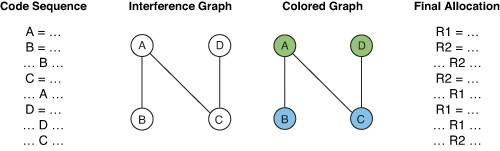
\includegraphics[scale=0.5]{figures/nshape}
\caption{Register Allocation via Graph Coloring}
\end{figure}
Find a {\bf \color{green} k-Coloring} for the interference graph, where {\bf \color{green} $k = \#\textsc{Registers}$}
\end{frame}

\subsection{Spilling}
\begin{frame}{Spilling}
	\begin{itemize}
		\item What if a \alert{k-Coloring} can't be found? Must {\bf \color{green} Spill} memory \\
		\qquad \\
		\item Simply insert new \alert{Load / Store} instructions as needed \\
		\qquad \\

		\item Potentially \alert{creates new bubbles} in the pipeline, need to re-perform scheduling \\
      \qquad \\
      
    \item Hence, in order to find an optimal schedule, \alert{Instruction
        Scheduling and Register Allocation must be performed together}. However
      this is a known {\bf \color{green}NP-Hard} problem
	\end{itemize}
\end{frame}

\section{Rapid Prototyping With Coconut}

\subsection{What Is COCONUT?}
\begin{frame}{Rapid Prototyping With Coconut}

	\alert{COCONUT}: (\alert{CO}de \alert{CON}structing \alert{U}ser \alert{T}ool) \\
	\begin{itemize}
	    \item COCONUT is an {\color{green} Interactive Development ToolSet}
        for performance critical assembly code, with existing implementations on
        {\color{green} PowerPC and Z}
	\end{itemize}

    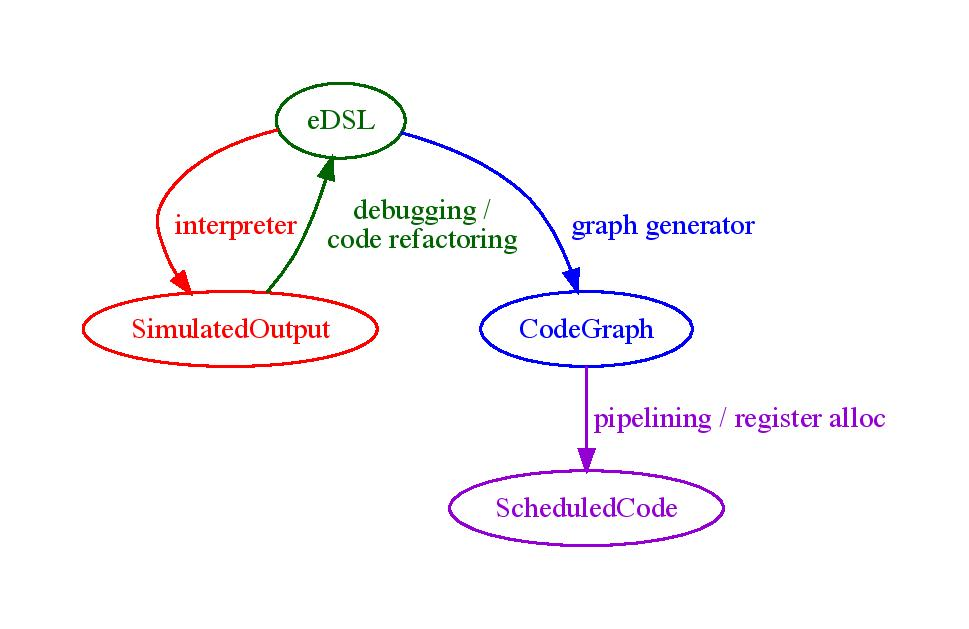
\includegraphics[scale=0.5]{figures/prototyping}
\end{frame}      

 \defverbatim[colored]\macrocode{
\begin{lstlisting}[language=haskell,tabsize=2]
#define INLINED_CODE(a0,b0,c0,..) \ 
vadd a0,b0,a0 \   
vsub a0,c0,a0 \  
...          
\end{lstlisting}}
   
 \defverbatim[colored]\coconutcode{
\begin{lstlisting}[language=haskell,tabsize=2]
some_func :: (VR n,GPR n,VR n,...) -> (MR n, VR n,...)
some_func (a0,b0,c0,...) = let
    a0_0 = vadd b0 a0
    a0_1 = vsub c0 a0_0
    ...
   in (a0_0,a0_1,...)  
\end{lstlisting}}
   
\begin{frame}{Rapid Prototyping With Coconut}

Performance critical assembly code can be encoded in the {\bf \color{green} Coconut eDSL},
an {\bf \color{green} IR Language} similar to LLVM. \\
\qquad \\
\alert{Example Coconut Code} \\
\coconutcode
\end{frame}

\begin{frame}{Example: Instruction Dependency DAG}
      \begin{figure}
        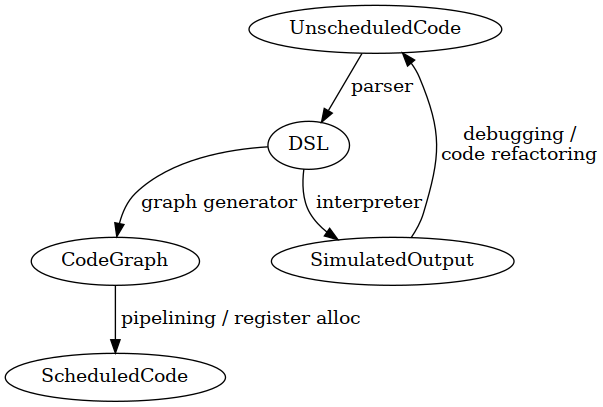
\includegraphics[scale=0.085]{figures/graph}
        \caption{Vector Instruction Dep. Graph}
      \end{figure}
    \end{frame}


\subsection{Why COCONUT?}
\begin{frame}{Why COCONUT?}
    
  Assembly programming is painful, COCONUT provides
    \qquad \\
    \begin{itemize}
            \item {\bf \color{green}A Domain Specific Language}: embedded in Haskell
            \item {\bf \color{green} Type Safety}: distinctly differentiates between Vector
              Registers and GPR's
            \item {\bf \color{green} Single Static Assignment (SSA)}: without consideration for {\bf register allocation / pipelining}
            \item {\bf \color{green} Simulation}: test code correctness with an
              integrated simulator
            \item {\bf \color{green}Continuous Optimization Based Scheduling}: a unique environment for
              implementing scheduling algorithms
        \end{itemize}    
\end{frame}

\section{Stochastic Scheduling Algorithm}

\subsection{Continouous Optimization Model}

\begin{frame}{Why Continuous Optimization Based Scheduling}

  Why Continuous Optimization?
  \begin{itemize}
  \item Scheduling may at first seem to be an inherently \alert{discrete} problem
  \item Compilers generally utilize \alert{heuristics} that are
    \alert{performed in passes} to discretely schedule instructions
  \item These heuristics may have a good premise, but tend to \alert{overwrite eachother} depending on the order performed
  \item By performing a \alert{relaxation to a continuous domain}, we
    create more leeway to find a happy middleground between heuristics
  \end{itemize}
\end{frame}

    \begin{frame}{Relaxed Continuous Optimization based Scheduling}
      Per Instruction $i$, perform a relaxation of scheduled position to dispatch and completion times $t_i$,$b_i$
      \begin{align*}
        \text{\color{cyan} Objective Variables \qquad} & t_i, b_i, f_i:& \mathbb{R} \\
        \text{\color{cyan} Constants \qquad} & \textrm{II} :& \mathbb{R} \\
        \text{\color{cyan} Indicator Function \qquad} & \mathbb{IN} :& \mathbb{R} \rightarrow \mathbb{R} \\
                                                       & t_i :& \text{dispatch time} \\
                                                       & b_i :& \text{completion time} \\
                                                       & f_i :& \text{FIFO use } 0 \leq f_i \leq 1 \\
                                                       & \textrm{II} :& \text{iteration interval} \frac{\# instructions}{dispatches/cycle} \\
      \end{align*}
      
    \end{frame}

    \begin{frame}{Relaxed Continuous Optimization based Scheduling}
      \begin{align}
        \text{\color{cyan} Hard Constraints \qquad}  & t_i + \epsilon \leq t_j \qquad & \forall i,j \cdot i \rightarrow j \\
                                                     & 0 \leq t_i \leq b_i \leq \#\text{stages} \cdot \textrm{II}  & \\
                                                     & b_i + \epsilon \leq t_i + \textrm{II} \\
        \text{\color{cyan} Objective Function \qquad}   & \text{min} \sum_{i} (b_i - t_i + f_i) + \text{Penalties}
      \end{align}
      
      {\bf \color{green} Key Idea:} Encode choice heuristics as penalties, adjust preference by between heuristics scaling
    \end{frame}

    \begin{frame}{Relaxed Continuous Optimization based Scheduling}
      
      {\bf \color{green} Other Key Idea:} Need to construct penalty to prevent \alert{Spilling}. Need to prevent clobbering of certain types of instructions \\
      {\bf \color{green} Solution:} Indicator function to detect penalize clobbering
      \begin{figure}
        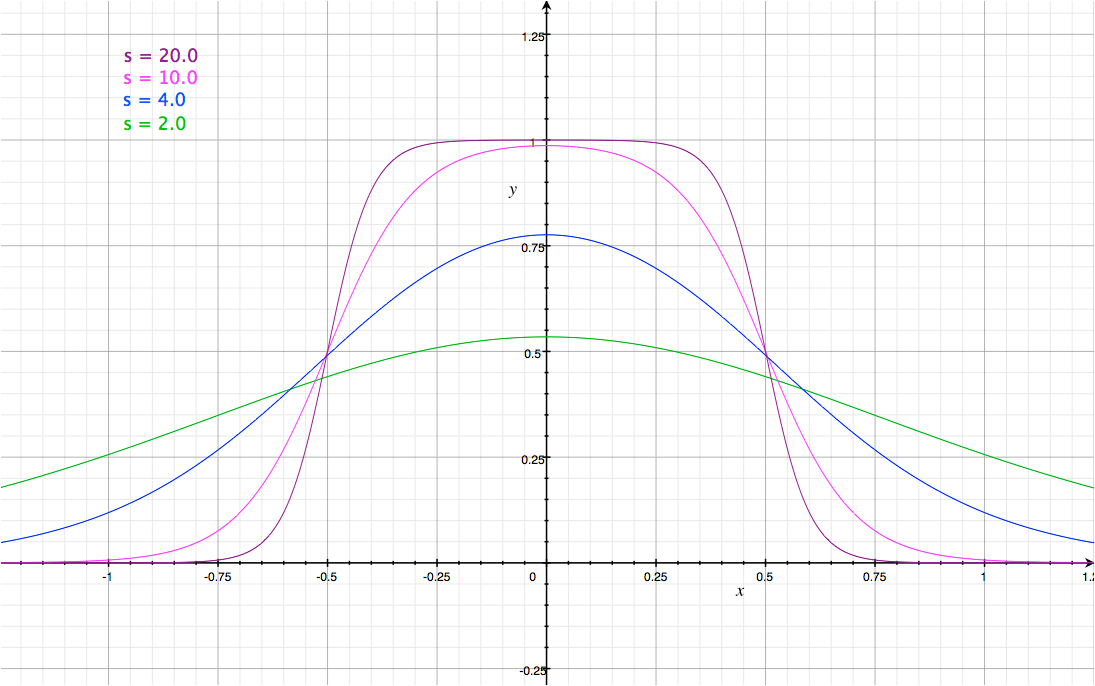
\includegraphics[scale=0.2]{figures/sigmoid}
        \caption{Altered Sigmoid Indicator Function}
      \end{figure}
    \end{frame}

    \subsection{Stochastic Parameterization}
    \begin{frame}{Sample Heuristic: IO Penalty}

      \begin{itemize}
        \item {\bf \color{green} IDEA}: penalize dispatch time of instruction
          based on the number and latency of it's dependencies

        \item {\bf \color{green} IO Penalty} \\

          \begin{align*}
            \text{\color{cyan} Given \qquad}  & t_i,t_j \qquad & \forall i,j \mid i \rightarrow j  \\
            \text{\color{cyan} For each i \qquad} & N_j  =  \sum_{i \rightarrow j} \text{latency}(j) & \\
            \qquad & \qquad & \qquad \\
            \qquad & \mathbb{IO}(i) = \sum_{j} \frac{1}{N_j} \mathbb{IN}(t_i - t_j) & \qquad 
          \end{align*}
          
      \end{itemize}
    \end{frame}

    \begin{frame}{Stochastic Scaling}

      \begin{itemize}
      \item The scaling $\frac{1}{N_j}$ may be a good \alert{guess}, but not
        necessarily effective in practice
      \item {\bf \color{green} IDEA} Scale the $\mathbb{IO}$ penalty
        stochastically \\
        \qquad \\

        
        \begin{align*}
          \text{\color{cyan} Define a Clustering} \qquad & \mathbb{C} = \text{Cluster}(\forall i \mid i \rightarrow j) \\
          \text{\color{cyan} For each Cluster i} \qquad & c_i \in \mathbb{RAND(R)} \\
          \text{\color{cyan} Stochastic Penalty} \qquad & \sum_i c_i \cdot \mathbb{IO}(i)
        \end{align*}

         {\bf \color{green} Note}: given a liberal clustering, generating schedules can \alert{span all schedules}
      \end{itemize}
    \end{frame}

    \section{Analysis}
    \begin{frame}{Parameter Estimation}

      \begin{itemize}
      \item \alert{Scaling Parameters} reflect how different
        groups of instructions interact with eachother \\
        \qquad \\
      \item These interactions will be specific to the kind of code we're
        scheduling and the architecture we're working with \\
        \qquad \\
      \item If we fix the optimization problem, and have \alert{ training
          data} from stochastically generated parameters, we can focus on
        \alert{Parameter Estimation} of our scalings
      \end{itemize}
    \end{frame}

    \begin{frame}{Principle Component Analysis}

      \begin{itemize}
        \item PCA is a statistical procedure commonly used  in data
          science to \alert{judge the importance of parameters} involved
          in a \alert{ predictive model}
        \item Performing PCA on the scaling parameters reveals the
          importance of commonly used instructions in relation to eachother
        \item This presents a new method of \alert{ analyzing the
            good and bad} of an architecture with respect to scheduling
      \end{itemize}
    \end{frame}
    
    %% #TODO DELETE ME 
    \begin{frame}{Questions?}
      
    \end{frame}
    
  \end{darkframes}

\end{document}
